\documentclass[12pt, twoside]{article}
\usepackage[letterpaper, margin=1in, headsep=0.2in]{geometry}
\setlength{\headheight}{0.6in}
%\usepackage[english]{babel}
\usepackage[utf8]{inputenc}
\usepackage{microtype}
\usepackage{amsmath}
\usepackage{amssymb}
%\usepackage{amsfonts}
\usepackage{siunitx} %units in math. eg 20\milli\meter
\usepackage{yhmath} % for arcs, overparenth command
\usepackage{tikz} %graphics
\usetikzlibrary{quotes, angles}
\usepackage{graphicx} %consider setting \graphicspath{{images/}}
\usepackage{parskip} %no paragraph indent
\usepackage{enumitem}
\usepackage{multicol}
\usepackage{venndiagram}

\usepackage{fancyhdr}
\pagestyle{fancy}
\fancyhf{}
\renewcommand{\headrulewidth}{0pt} % disable the underline of the header
\raggedbottom
\hfuzz=2mm %suppresses overfull box warnings

\usepackage{hyperref}

\fancyhead[LE]{\thepage}
\fancyhead[RO]{\thepage \\ Name: \hspace{4cm} \,\\}
\fancyhead[LO]{BECA / Dr. Huson / Geometry\\*  Unit 3: Parallel lines and transversals\\* 12 October 2022}

\begin{document}

\subsubsection*{3.2 Finding angle measures for transverse lines}
\begin{enumerate}

\item Given two parallel lines and a transversal, with $m\angle 4 = 3x$ and $m\angle 5 = x + 70$. \\ Write an equation, then solve for $x$.
\begin{flushright}
  \begin{tikzpicture}[scale=1]
    \draw [<->, thick] (3,2)--(8,2);
    \draw [<->, thick] (2,0)--(7,0);
    \draw [<->, thick] (4,-1)--(5.5,3);
    \node at (4.5,0.3) [left]{$5$};
    \node at (4.5,0.3) [right]{$6$};
    \node at (4.3,-0.3) [left]{$7$};
    \node at (4.3,-0.3) [right]{$8$};
    \node at (5.2,2) [above left]{$1$};
    \node at (5.2,2) [above right]{$2$};
    \node at (5,2) [below left]{$3$};
    \node at (5,2) [below right]{$4$};
  \end{tikzpicture}
\end{flushright} \vspace{2cm}

\item Given two parallel lines and a transversal, with $m\angle 1 = 3x-10$ and $m\angle 8 = 2x + 32$. \\ Write an equation, then solve for $x$.
\begin{flushright}
  \begin{tikzpicture}[scale=1]
    \draw [<->, thick] (3,2)--(8,2);
    \draw [<->, thick] (2,0)--(7,0);
    \draw [<->, thick] (4,-1)--(5.5,3);
    \node at (4.5,0.3) [left]{$5$};
    \node at (4.5,0.3) [right]{$6$};
    \node at (4.3,-0.3) [left]{$7$};
    \node at (4.3,-0.3) [right]{$8$};
    \node at (5.2,2) [above left]{$1$};
    \node at (5.2,2) [above right]{$2$};
    \node at (5,2) [below left]{$3$};
    \node at (5,2) [below right]{$4$};
  \end{tikzpicture}
\end{flushright} \vspace{1cm}

\item Do Now: Given two parallel lines and a transversal, as shown, with $m\angle 8 = 123^\circ$.
  \begin{multicols}{2}
    \begin{enumerate}[itemsep=0.5cm]
      \item What angle is corresponding to $\angle 8$?
      \item What angle is alternate exterior to $\angle 8$?
      \item Find $m\angle 2$ \vspace{1cm}
    \end{enumerate}
    \begin{flushright}
      \begin{tikzpicture}[scale=1,rotate=20]
      \draw [<->, thick] (3.5,2)--(7,2);
      \draw [<->, thick] (2.5,0)--(6,0);
      \draw [<->, thick] (4,-1)--(5.5,3);
      \node at (4.5,0.3) [left]{$5$};
      \node at (4.5,0.3) [right]{$6$};
      \node at (4.3,-0.3) [left]{$7$};
      \node at (4.3,-0.3) [right]{$8$};
      \node at (5.2,2) [above left]{$1$};
      \node at (5.2,2.1) [above right]{$2$};
      \node at (5,2) [below left]{$3$};
      \node at (5.1,2) [below right]{$4$};
    \end{tikzpicture}
  \end{flushright}
  \end{multicols}

\item Find $m\angle 1$ given two parallel lines and a transversal, with
  \begin{multicols}{2}
  $\displaystyle m\angle 2 = \frac{2}{7}(2x+58)$ \hspace{0.75cm}$\displaystyle m\angle 7 = \frac{1}{7}(5x+5)$
\begin{flushright}
  \begin{tikzpicture}[scale=1,rotate=-10]
    \draw [<->, thick] (3,2)--(8,2);
    \draw [<->, thick] (2,0)--(7,0);
    \draw [<->, thick] (4,-1)--(5.5,3);
    \node at (4.5,0.3) [left]{$5$};
    \node at (4.5,0.3) [right]{$6$};
    \node at (4.3,-0.3) [left]{$7$};
    \node at (4.3,-0.3) [right]{$8$};
    \node at (5.2,2) [above left]{$1$};
    \node at (5.4,2) [above right]{$2$};
    \node at (4.9,2) [below left]{$3$};
    \node at (5,2) [below right]{$4$};
  \end{tikzpicture}
\end{flushright} 
\end{multicols} \vspace{2cm}

\newpage
\item Two parallel lines intersect a transversal. Given corresponding angles  $m\angle 1 = 4.4x - 63$ and $m\angle 2 = 2.8x+9$, find the measure of $\angle 1$. 
  \begin{flushright}
    \begin{tikzpicture}[scale=0.9]
      \draw [<->, thick] (3,0)--(9,0);
      \draw [<->, thick] (2,2)--(8,2);
      \draw [<->, thick] (5,-1)--(3,3);
      %\draw [<->, thick] (11,-1)--(9,3);
      %\node at (4, 1.7){$1$};
      \node at (5.3, 2.25){$m\angle 1 = 4.4x - 63$};
      \node at (6.1, 0.25){$m\angle 2 = 2.8x+9$};
      %\node at (10, 0.25){$3$};
    \end{tikzpicture}
    \end{flushright}

\item Given two parallel lines and a transversal, with $m\angle 3 = 18(x-1)$ and $m\angle 5 = 18(x+1)$. Find $m\angle 1$. (First write an equation, and solve for $x$)
  \begin{flushright}
  \begin{tikzpicture}[scale=1,rotate=-10]
    \draw [<->, thick] (3,2)--(8,2);
    \draw [<->, thick] (2,0)--(7,0);
    \draw [<->, thick] (4,-1)--(5.5,3);
    \node at (4.5,0.3) [left]{$5$};
    \node at (4.5,0.3) [right]{$6$};
    \node at (4.3,-0.3) [left]{$7$};
    \node at (4.3,-0.3) [right]{$8$};
    \node at (5.2,2) [above left]{$1$};
    \node at (5.4,2) [above right]{$2$};
    \node at (4.9,2) [below left]{$3$};
    \node at (5,2) [below right]{$4$};
  \end{tikzpicture}
\end{flushright} \vspace{1cm}


\item Find $m\angle 1$ given two parallel lines and a transversal, with
\begin{multicols}{2}
$\displaystyle m\angle 4 = 10(7x-4)$ \hspace{0.75cm}$\displaystyle m\angle 6 = 8(7x-4)$
\begin{flushright}
\begin{tikzpicture}[scale=1,rotate=-10]
  \draw [<->, thick] (3,2)--(8,2);
  \draw [<->, thick] (2,0)--(7,0);
  \draw [<->, thick] (4,-1)--(5.5,3);
  \node at (4.5,0.3) [left]{$5$};
  \node at (4.5,0.3) [right]{$6$};
  \node at (4.3,-0.3) [left]{$7$};
  \node at (4.3,-0.3) [right]{$8$};
  \node at (5.2,2) [above left]{$1$};
  \node at (5.4,2) [above right]{$2$};
  \node at (4.9,2) [below left]{$3$};
  \node at (5,2) [below right]{$4$};
\end{tikzpicture}
\end{flushright} 
\end{multicols}

\end{enumerate}
\end{document}